%
% ---------- header -----------------------------------------------------------
%
% project       kaneton
%
% license       kaneton
%
% file          /home/mycure/kaneton/view/book/assignments/future/k1.tex
%
% created       julien quintard   [fri nov 28 05:25:37 2008]
% updated       julien quintard   [fri nov 28 05:35:29 2008]
%

%
% ---------- k1 ---------------------------------------------------------------
%

\chapter{k1}
\label{chapter:k1}

\name{k1} consists in the development of the memory management system.

\newpage

%
% ---------- text -------------------------------------------------------------
%

%
% objectives
%

\section{Objectives}

This project aims at learning advanced memory management in operating systems. Students will learn how to deal with MMU and Cache entries (TLB) through the concepts of Physical Memory, Virtual Memory and Address Space.

The students will also have to implement a memory allocator, with the algorithm of their choice. The performance of the allocator will be tested.

%
% requirements
%

\section{Requirements}

The students must know the concepts of Physycal and Virtual memory and the mapping techniques. Especially the paging technique must be known since it is what has to be implemented. Since this implementation will be tested on the ia32 architecture, the students will need the Intel documentation so they can find how to interface with the MMU.

%
% snapshot
%

\section{Snapshot}

There are 3 main managers in the kaneton design that are used to handle memory :

\begin{itemize}
\item \textbf{segment :} In the kaneton terminology, a segment is a block of physical memory. The segment manager handles the allocation of blocks in the physical memory, provides methods to read and write these blocks, and to set permissions on these blocks. Please note that this is not related to the Intel segment concept.

\item \textbf{region :} In the kaneton terminology, a region is a block of virtual memory. The region manager handles the allocation of blocks in the virtual memory as well as the mapping of these blocks to kaneton segments, and provides methods to read, write, and set permissions on these blocks. Please note that the region manager will never reserve a segment by itself, allocating a region requires to provide a valid, already allocated, segment.

\item \textbf{map :} The map manager in kaneton is a higher level interface that handles memory allocation. It will reserve a segment, and will map a region on the segment with a single call.
\end{itemize}

%
% assignments
%

\section{Assignments}

\subsection*{Abstract}

The segment manager and the map manager are already provided in the snapshot. The students will have to implement the region manager completely.

A region designs a block of virtual memory, so it is a quite generic concept. Some of the work to be done is therefore architecture dependant, but since it also consists in dealing with the MMU mappings, some part of it is architecture dependant.

Kaneton is a portable kernel, so each module has been designed to have an independant code and several dependant code, one for each architecture. The sudents will have to think about which code should go in the independant or in the dependant part. Please note that some functions may only have independant code.

\subsection*{Files}

\begin{tabular}{| l | l |}
  \hline
  machine-independent & {\em kaneton/core/region/region.c}\\\hline
  machine-independent & {\em kaneton/core/region/region-fit.c}\\\hline
  machine-dependent & {\em kaneton/machine/glue/ibm-pc.ia32/educational/region.c}\\\hline
\end{tabular}

\subsection*{Required implementation}

\function{t\_error}{region\_initialize}{\type{t\_vaddr} \argument{start},
					\type{t\_vsize} \argument{size}}
{
  This function initializes the region manager. The virtual addresses that can
  be returned by the allocator must be in the range defined by \argument{start}
  and \argument{size}.
}

\function{t\_error}{region\_clean}{\type{void}}
{
  This function releases the ressources of the region manager.
}

\function{t\_error}{region\_space}{\type{i\_as} \argument{asid},
				   \type{t\_vsize} \argument{size},
				   \type{t\_vaddr*} \argument{address}}
{
  This function tries to find \argument{size} bytes of free space in the
  address space \argument{asid}. The base address of the free block found
  by \code{region\_space} is returned through the \argument{address} parameter.
  
  \-
  
  The allocation algorithm is up to you.
  First fit is probably the easier one, but you can implement a more
  complex algorithm such as a buddy system, for example. The performance of
  your implementation will be tested.
}

\function{t\_error}{region\_reserve}{\type{i\_as} \argument{asid},
				     \type{i\_segment} \argument{segid},
				     \type{t\_paddr} \argument{offset},
				     \type{t\_opts} \argument{opts},
				     \type{t\_vaddr} \argument{address},
				     \type{t\_vsize} \argument{size},
				     \type{i\_region*} \argument{regid}}
{
  This function reserves a region of size \argument{size} in the address space
  \argument{asid} and maps the segment \argument{segid} to it. The identifier
  of this new region object is returned through the \argument{regid} parameter.
  
  \-
  
  The values for \argument{opts} can be:
  \begin{itemize}
    \item REGION\_OPT\_NONE: no options
    \item REGION\_OPT\_FORCE: force the region to be reserved at virtual
      address \argument{address}. Otherwise, it uses \code{region\_space} to
      determine the address.
    \item REGION\_OPT\_USER: The region will be addressable both in the user
      and kernel mode.
    \item REGION\_OPT\_PRIVILEGED: The region will only be addressable in the
      kernel mode.
    \item REGION\_OPT\_LOCAL: The region will be local to the address space
      specified by \argument{asid}
    \item REGION\_OPT\_GLOBAL: The region will be global to all the address
      spaces.
  \end{itemize}
  \argument{offset} specifies the offset in the segment where the mapping of the region occurs, so that reserving several regions on the same segment is possible.
  \begin{center}
    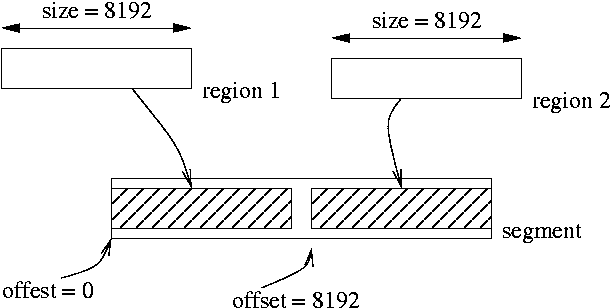
\includegraphics[width=0.4\linewidth]{figures/k1-offset}
  \end{center}

}

\function{t\_error}{region\_release}{\type{i\_as} \argument{asid},
				     \type{i\_region} \argument{regid}}
{
  This function releases the region \argument{regid} that belongs to the
  address space \argument{asid}.
}

\function{t\_error}{region\_inject}{\type{i\_as} \argument{asid},
                                    \type{o\_region*} \argument{o},
				    \type{i\_region*} \argument{regid}}
{
  This function injects the region \argument{o} into the address space
  \argument{asid}. 
}

\function{t\_error}{region\_split}{\type{i\_as} \argument{asid},
				   \type{i\_region} \argument{regid},
				   \type{t\_vsize} \argument{size},
				   \type{i\_region*} \argument{left},
				   \type{i\_region*} \argument{right}}
{
  This function splits the region \argument{regid} in two regions returned
  through the parameters \argument{left} and \argument{right}, in the address
  space \argument{asid}. The parameter \argument{size} defines the new size
  for the \argument{left} region, the \argument{right} region will take the
  remaining space.  
}

\function{t\_error}{region\_resize}{\type{i\_as} \argument{as},
				    \type{i\_region} \argument{old},
				    \type{t\_vsize} \argument{size},
				    \type{i\_region*} \argument{new}}
{
  This function resizes the region \argument{old} of the address space
  \argument{asid}. The new size is specified in \argument{size} and the resized
  region is returned through the parameter \argument{new}.
}

\function{t\_error}{region\_coalesce}{\type{i\_as} \argument{asid},
                                      \type{i\_region} \argument{left},
				      \type{i\_region} \argument{right},
				      \type{i\_region*} \argument{regid}}
{
  This function merges two adjacent regions \argument{left} and
  \argument{right}, in the address space \argument{asid}. The resulting new
  region is returned through the parameter \argument{regid}.
}

\function{t\_error}{region\_flush}{\type{i\_as} \argument{asid}}
{
  This function releases all the regions of the address space \argument{asid}.
}

\function{t\_error}{region\_get}{\type{i\_as} \argument{asid},
				 \type{i\_region} \argument{regid},
				 \type{o\_region**} \argument{o}}
{
  This function returns the region object from its id \argument{regid} and the
  address space \argument{asid}, through the parameter \argument{o}.
}

\subsection*{Optional implementation}

The following functions are not going to be tested by our test suite, you are
not forced to do them although we strongly recommend you to do it, since they
are very helpful for debugging your implementation.

\-

Since this is not tested, the output format is up to you.

\function{t\_error}{region\_show}{\type{i\_as} \argument{asid},
                                  \type{i\_region} \argument{regid}}
{
  This function displays the region object specified by its id \argument{regid}
  and the address space \argument{asid}.
}

\function{t\_error}{region\_dump}{\type{i\_as} \argument{asid}}
{
  This function displays all the region objects that belong to the address
  space \argument{asid}.
}

\subsection*{Important}
Please note that you have the independant and the dependant part to do.
All the functions might not require an dependant part though. The dependant
part file doesn't contain any prototypes. It's your responsability to add a
dependant function if you think it needs one.

\-

Some structures relative to the region manager are already provided, but you
are free to modify them if you want to. You can freely add new fields, and also
modify the existing ones, but in that case, it's your responsibility to make
changes in the code so that everything still works.
